% Template for ICIP-2022 paper; to be used with:
%          spconf.sty  - ICASSP/ICIP LaTeX style file, and
%          IEEEbib.bst - IEEE bibliography style file.
% --------------------------------------------------------------------------
\documentclass{article}
\usepackage{spconf,amsmath,graphicx, booktabs, appendix, float}
\usepackage{amsfonts}
\usepackage[hidelinks]{hyperref} % must be last
\usepackage[section]{placeins}



% Example definitions.
% --------------------
\def\x{{\mathbf x}}
\def\L{{\cal L}}

% Title.
% ------
\title{Transfer Learning for Multi-label Retinal Disease Classification \thanks{\textit{Code available at \url{github.com/littlemicrowave/Multi-Retinal-Disease-Detection}}}}
%
% Single address.
% ---------------
%\name{Leo Davidov, Seyyedhamid Azimidokht\thanks{Thanks to XYZ agency for funding.}}
%\address{Author Affiliation(s)}
%
% For example:
% ------------
%\address{School\\
%	Department\\
%	Address}
%
% Two addresses (uncomment and modify for two-address case).
% ----------------------------------------------------------
\twoauthors
{Leo Davidov}
{University of Oulu\\
Leo.Davidov@student.oulu.fi}
{Seyyedhamid Azimidokht}
{University of Oulu\\
Seyyedhamid.Azimidokht@oulu.fi}

\begin{document}
%\ninept
%
\maketitle
%
\section{Introduction}
\label{sec:intro}

Retinal diseases often share visual characteristics, making both single- and multi-label classification challenging, particularly under limited and imbalanced data. Deep learning methods have shown strong performance in medical image analysis, but their effectiveness heavily depends on data availability.

In this project, we address the problem of multi-label retinal disease detection, focusing on three major conditions: Diabetic Retinopathy (DR), Glaucoma (G), and Age-related Macular Degeneration (AMD). 

To tackle the challenge of limited annotated medical data we examine various data augmentation methods, class balancing, architectural tweaks, and adopt transfer learning strategies, leveraging models pretrained on large-scale datasets and fine-tuning them for multi-label retinal image classification.

\section{Methods}

\subsection{Data and preprocessing}

Experiments are conducted using the sample from ODIR dataset  \cite{Li2020OcularBenchmark}, which is divided into a training set, a validation set, an off-site test set, and an on-site test set of 250 images. Images were then resized to a fixed resolution 256$\times$256, 224$\times$224, or 128$\times$128, and normalized using ImageNet \cite{Deng2009ImageNet} statistics, or using mean of 0.5 and standard deviation 0.5 depending on the experiment. Distribution of class labels in the corresponding sets can be found from Table~\ref{tab:data_distrib}.

\subsection{Backbone models}

We evaluated EfficientNetB0~\cite{Tan2019EfficientNet} and ResNet18~\cite{He2016ResNet} as backbone architectures pretrained on large ophthalmic datasets, including ADAM~\cite{Fang2022ADAM}, REFUGE2~\cite{Fang2022REFUGE2}, and APTOS~\cite{APTOS2019}. In addition, we evaluated ImageNet-pretrained vision transformer backbones, including TinyViT~\cite{Wu2022TinyViTArXiv} and the hierarchical SwinV2-Tiny~\cite{Liu2022SwinV2}. We have employed a two-staged fine-tuning, by first training replaced layers while the backbone is frozen, and later fine-tuning the full updated model.

\subsection{Attention mechanisms}

Apart from replacing the classifier head of pretrained backbones with the fully connected linear layer with 3 logits according to multi-label classification of 3 targets, we examined the performance impact of attention mechanisms, in particular by appending one Squeeze-and-Excitation (SE) \cite{Hu2018SENet} block and Multi-head-Attention (MHA) \cite{Vaswani2017Attention} layer to the ResNet and EfficientNet.

For SE, a reduction ratio of $r=16$ was used, with a minimum bottleneck dimension of 1. Multi-head self-attention was implemented via a transformer block with relative positional encoding (RPE)~\cite{Shaw2018RelativeAttention}, with 2D relative spatial offsets being capped to a maximum distance of $\pm3$, with input channels, as well as  $Q$, $K$, and $V$ being linearly projected to dimension $D=128$ for ResNet and $D=256$ for EfficientNet, and split into four attention heads. The attention output was projected back to the input dimensionality and followed by dropout with rate 0.2. The final result was obtained via a scaled residual connection followed by layer normalization:
\begin{equation}
Y = \mathrm{LayerNorm}(X + \alpha O),
\end{equation}
where $\alpha$ is a learnable scaling parameter, so during fine-tuning model could adjust how much self-attention it needs, we initialized it by default to 0.5.

\subsection{Data Augmentation}

To mitigate data scarcity and class imbalance, several data augmentation techniques were employed, including color jittering (brightness, saturation, hue), rotations $\pm90$, and noise injection into images during TinyViT and SwinV2-Tiny tuning. All augmentations were applied online during training to increase data diversity and improve model generalization.

Apart from conventional augmentation, we evaluated the generation of class-conditional fundus images using variational autoencoders (VAEs) \cite{Kingma2013VAE} and deep convolutional generative adversarial networks (DCGAN) \cite{Radford2015DCGAN}.

For the VAE, a pretrained ResNet18 was used as the encoder, while the decoder was implemented using residual upsampling convolutions following the design principles of the BigGAN generator \cite{Brock2018BigGAN}. Class conditioning was incorporated using Feature-wise Linear Modulation \cite{Perez2018FiLM}, replacing the affine parameters in batch normalization layers; the same conditioning mechanism was applied to the DCGAN generator. In addition, the original DCGAN architecture was modified by reducing the capacity of both generator ($G$) and discriminator ($D$) approximately twice, accounting to the dataset size, and instead of batch normalization in the $D$, spectral normalization was employed, which normalizes layer weight matrices using their largest singular values, enforcing Lipschitz constraint, and has been shown to improve discriminator training stability in GANs, including BigGAN. For $D$ conditioning, we adopted a projection-based formulation \cite{Miyato2018ProjectionDiscriminatorArXiv}, and have also employed an auxiliary classification head following the idea of AC-GAN \cite{Odena2016ACGANArXiv}.

For training TinyViT, SwinV2-Tiny, and our conditional VAE and GAN implementations we also included weighted random sampling with replacement (RSWR) as an additional augmentation and class balancing strategy.

\subsection{Loss functions}
\label{sec:losses}
The ODIR dataset exhibits strong class imbalance. To address this, we experimented with three loss re-weighting strategies: 
(i) weighted binary cross-entropy (WBCE), where the loss for each class was scaled by the ratio of negative to positive samples, (ii) Class-Balanced Loss (CB) \cite{cui2019class}, which reweights each label using the effective number of samples with $\beta=0.999$, and finally, (iii) Focal Loss \cite{lin2017focal} which operates at the prediction level by down-weighting easy examples within each sample, with focusing parameter set to $\gamma=2$ and a class-balancing factor $\alpha=0.75$.

For the VAE, we optimized the classical Evidence Lower Bound (ELBO) under class conditioning formulation, with gradually increasing $\beta$ factor for KL Divergence:
\begin{equation}
\mathcal{L}_{\text{ELBO}}
=
-\mathcal{L}_{\text{rec}}
-
\beta\mathrm{KL}\!\left(q_\phi(z\mid x,y)\,\|\,p(z)\right),
\end{equation}
where $\mathcal{L}_{\text{rec}}$ denotes the reconstruction loss, implemented as BCE over pixel intensities across the three color channels, corresponding to a Bernoulli likelihood.

For GAN training, we employed a Hinge loss \cite{Brock2018BigGAN, Miyato2018ProjectionDiscriminatorArXiv} with an auxiliary BCE loss for classifer head of $D$ with $\alpha=0.5$, considering our multi-label nature of data:
\begin{equation}
\begin{aligned}
\mathcal{L}_{D}
&=
\max(0, 1 - D(x))
+
\max(0, 1 + D(G(z)))
\\
&\quad +
\alpha\mathcal{L}_{\mathrm{BCE}}\!\left(C(x),y\right)
\end{aligned}
\end{equation}
\begin{equation}
\begin{aligned}
\mathcal{L}_{G}
&=
- D(G(z))
+
\alpha\,\mathcal{L}_{\mathrm{BCE}}\!\left(C(G(z)),y\right).
\end{aligned}
\end{equation}

Following exemplary explanation-based learning \cite{hagos2023learning}, we augment the classification loss with a triplet-based explanation loss that operates on Grad-CAM explanations. Given an input image $x$, its Grad-CAM map $\mathrm{CAM}(x)$, and two fixed exemplary explanations $C_{\text{good}}$ and $C_{\text{bad}}$, the explanation loss is defined as
\begin{equation}
\begin{aligned}
\mathcal{L}_{\text{expl}}
&=
\max\!\Big(
d(x \odot \mathrm{CAM}(x), C_{\text{good}})
-
\\
&\qquad\quad
d(x \odot \mathrm{CAM}(x), C_{\text{bad}}) + m,\; 0
\Big)
\end{aligned}
\end{equation}
where $d(\cdot,\cdot)$ denotes the Euclidean distance and $m=1$ is the margin. The final training objective is
\begin{equation}
\mathcal{L}
=
\mathcal{L}_{\mathrm{BCE}}
+
\alpha\,\mathcal{L}_{\text{expl}},
\end{equation}
with weighting coefficient $\alpha$. Further details on the construction of $C_{\text{good}}$, $C_{\text{bad}}$, and their use with Grad-CAM are provided later on.

\subsection{Grad-CAM}
We adopted the exemplary explanation-based learning framework (eXBL) \cite{hagos2023learning}, which refines model explanations using a small set of representative Grad-CAM exemplars. Grad-CAM explanations are computed using the fully fine-tuned baseline model from Task~1 (the unrefined model).

For each disease class, we select one good and one bad exemplar, denoted $C_{\text{good}}$ and $C_{\text{bad}}$, from the training set. Candidate explanations are ranked using the Activation Recall (AR) metric, which measures the overlap between Grad-CAM activations and relevant image regions (eye region mask), and the exemplars are chosen as those with the highest and lowest AR scores, respectively. Following \cite{hagos2023learning}, exemplars are defined as the element-wise product of the input image and its Grad-CAM map. AR is defined as
\begin{equation}
\mathrm{AR}(x)
=
\frac{\sum \left(\mathrm{CAM}(x) \odot M\right)}{\sum M},
\end{equation}

During training (refining), these class-specific exemplars are incorporated via the triplet-based explanation loss described in Section~\ref{sec:losses}.


\section{Results}
\subsection{ResNet and EfficientNet}
We are putting the most emphasis on the weighted-F1 and macro-F1, considering the multi-label nature of targets. We are reporting the stable on-site macro F1 scores for each experiment, supplied with corresponding detailed full tuning off-site evaluation (Appendix \ref{app:metrics}). We additionally provide fine-tuning schedules for each setup for reproducibility (Appendix \ref{app:settings}).

Performance of pretrained ResNet18 and EfficientNetB0 backbones was first evaluated without applying any class-balancing strategies, using only the standard BCE loss. On-site results are summarized in table below:

\begin{table}[H]
\centering
\begin{tabular}{lccc}
    \toprule
    \textbf{Model} & \textbf{No tuning} & \textbf{Head tuning} & \textbf{Full tuning}\\
    \midrule
    EfficientNetB0 & 60.22 & 73.71 & 81.24 \\
    ResNet18 & 56.92 & 62.56 & 81.07\\
    \bottomrule
\end{tabular}
\caption{Onsite F1-macro scores (\%)}
\label{tab:onsite_task1}
\end{table}
By default EfficientNet gives better performance results, showing architectural advantages in representation efficiency, but with full tuning, both models achieve comparable macro F1-scores on-site. Off-site ResNet showed 3-4\% better performance in macro and weighted F1 in our training setup, considering full-tuning output.

Incorporating an additional SE block into the convolutional backbones resulted in an on-site macro F1-score of 82\% for EfficientNet, with a ResNet having a negligible negative difference to this scoring. Indicating that even simple additional channel-wise recalibration helps to emphasize disease-relevant features in multi-label retinal classification. On off-site evaluation, ResNet architecture gave slightly better results with 1\% difference.

Multi-head self-attention, which was implemented as the part of the transformer block with RPE and residual connection, improved the baseline performances of both models with the EfficientNet backbone achieving 82.29\% on-site and the best off-site weighted F1 among all experiments of 86\%, with ResNet having almost identical results.

Further, we evaluated loss re-weighting strategies to mitigate class imbalance, with no modifications applied to the backbones. The performance difference between the two models was not significant. Nevertheless, Focal Loss obtained its best result with ResNet at 81.58\% on-site. WBCE delivered the largest improvement overall, in comparison to the original CB formulation, achieving the on-site macro F1-score of 84.13\% with ResNet as well, indicating the effectiveness of frequency-based re-weighting in this multi-label setting.

Visual inspection of Grad-CAM overlays (Fig~\ref{fig:grad-cam-augment}) revealed that the models often attend to regions outside the eye area. To mitigate this, we applied noise augmentation to the non-eye regions, which yielded an on-site macro F1-score of 81.2\%  for EfficientNet, while also improving off-site generalization.

Incorporating explanation-based supervision using Grad-CAM and the proposed triplet explanation loss further improved model performance. Using class-specific exemplary explanations selected from the training set, the model EfficientNet achieved an on-site macro F1-score of 82.7\%, demonstrating that aligning model attention with anatomically meaningful regions can benefit both interpretability and classification performance.


\subsection{Generative models}
Both models were trained for a target resolution 128x128. cVAE encoder was frozen for the first 15 epochs. The latent posterior didn't fully collapse to $\mathcal{N}(0,1)$, instead learned distribution had a $\mu$ close to 0 and a $\sigma$ of approximately 0.85. For cDCGAN, we performed noise injection into real images for the first 500 epochs to mitigate $D$ overconfidence. Learning rates were adjusted periodically throughout training to maintain stability.

cDCGAN-generated images are significantly sharper with more visible class conditioning than those produced by sampling cVAE posterior (Appendix \ref{app:figures}). However, outputs from both generative models were of insufficient quality for effective dataset augmentation, with limited anatomical detail. Additional experiments with different resolutions and patch-based $D$, and architectural tweaks, did not yield any benefit.

\subsection{Vision Transformers}
SwinV2-Tiny achieved an on-site macro F1-score of 82.40\%, and the best off-site macro F1 among reported results, with the highest precision-recall for AMD class, slightly outperforming TinyViT. SwinV2-Tiny supports direct 256x256 inputs, and has twice more capacity, unlike the employed TinyViT with 224x224. Swin architecture uses window-based self-attention, where attention is computed locally within shifted windows, which significantly reduces computational cost while preserving locality. Here we employed weighted RSWR, and augmentation described in Section 2.4.

\section{Discussion}

ResNet and EfficientNet have only minor difference in absolute performance. EfficientNet employs compound scaling and MBConv blocks with SE, twice smaller than ResNet, while ResNet benefits from residual skip connections, enabling stable gradient flow. Given the limited amount of data, EfficientNet is better suited. However, when considering relative performance gains over baseline values, architectural modifications such as MHA, SE, or alternative losses provide more improvement for ResNet (3–4\% on-site). ImageNet-pretrained Tiny Swin, and Tiny ViT demonstrated fast and stable fine-tuning with data augmentation, achieving competitive performance within 20–30 epochs.

Among all strategies, WBCE proved to be the most effective, offering the best trade-off between simplicity and performance improvement, as well as conventional data augmentation methods. MHA in the final layer significantly increased parameter count with limited benefit, in comparison to SE, so a compact transformer block was employed to mitigate that problem. Grad-CAM inspection exposed non-eye attention, and Grad-CAM–based triplet supervision further improved attention alignment and performance. In contrast, image generation using VAEs and GANs was ineffective due to limited data. It was very optimistic to expect high fidelity with 800 training images. VAE was initially an inappropriate solution, due to it's probabilistic formulation, which results in blurry outputs with loss of necessary detail in medical imaging. Potential solution could be two staged generation pipeline employing SRGAN for image refinement, or more complex models such as diffusion-based or CVAE-GAN hybrids. -------Workload distribution: 50\%-50\%





\clearpage
\vfill\pagebreak

% References should be produced using the bibtex program from suitable
% BiBTeX files (here: strings, refs, manuals). The IEEEbib.bst bibliography
% style file from IEEE produces unsorted bibliography list.
% -------------------------------------------------------------------------
\bibliographystyle{IEEEbib}
\bibliography{strings,refs}
\appendices

\section{Additional Tables}
\label{app:metrics}
\counterwithin{table}{section}
\begin{table}[H]
\centering
\begin{tabular}{lcccc}
    \toprule
    \textbf{Set} & \textbf{DR} & \textbf{G} & \textbf{AMD} & \textbf{Total Samples}\\
    \midrule
    Training set & 517 & 163 & 142 & 800 \\
    Validation set & 109 & 58 & 44 & 200  \\
    Offsite test set & 140 & 49 & 22 & 200 \\
    Onsite test set & - & - & - & 250\\
    \bottomrule
\end{tabular}
\caption{Label count distribution in ODIR sample.}
\label{tab:data_distrib}
\end{table}



\begin{table}[H]
\centering
\begin{tabular}{lccc}
\toprule
\textbf{Class} & \textbf{Precision} & \textbf{Recall} & \textbf{F1-score} \\
\midrule
DR   & 0.88 & 0.87 & 0.88 \\
G    & 0.82 & 0.65 & 0.73 \\
AMD  & 0.59 & 0.59 & 0.59 \\
\midrule
Macro avg    & 0.77 & 0.71 & 0.73 \\
Weighted avg & 0.84 & 0.79 & 0.81 \\
\bottomrule
\end{tabular}
\caption{Bare EfficientNetB0 full-tuning offsite.}
\label{tab:efficient_full_task1}
\end{table}

\begin{table}[H]
\centering
\label{tab:resnet18_full_task1}
\begin{tabular}{lccc}
\toprule
\textbf{Class} & \textbf{Precision} & \textbf{Recall} & \textbf{F1-score} \\
\midrule
DR  & 0.88 & 0.91 & 0.90 \\
G   & 0.85 & 0.71 & 0.78 \\
AMD & 0.61 & 0.64 & 0.62 \\
\midrule
Macro avg    & 0.78 & 0.75 & 0.77 \\
Weighted avg & 0.85 & 0.84 & 0.84 \\
\bottomrule
\end{tabular}
\caption{Bare ResNet18 full-tuning offsite.}
\label{tab:resnet18_full_task1}
\end{table}

\begin{table}[H]
\centering
\begin{tabular}{lccc}
\toprule
\textbf{Class} & \textbf{Precision} & \textbf{Recall} & \textbf{F1-score} \\
\midrule
DR  & 0.87 & 0.92 & 0.90 \\
G   & 0.87 & 0.67 & 0.76 \\
AMD & 0.65 & 0.59 & 0.62 \\
\midrule
Macro avg    & 0.80 & 0.73 & 0.76 \\
Weighted avg & 0.85 & 0.83 & 0.84 \\
\bottomrule
\end{tabular}
\caption{ResNet18 with WBCE offsite.}
\label{tab:resnet_cb_task3}
\end{table}


\begin{table}[H]
\centering
\begin{tabular}{lccc}
\toprule
\textbf{Class} & \textbf{Precision} & \textbf{Recall} & \textbf{F1-score} \\
\midrule
DR  & 0.87 & 0.94 & 0.90 \\
G   & 0.86 & 0.76 & 0.80 \\
AMD & 0.63 & 0.55 & 0.59 \\
\midrule
Macro avg    & 0.79 & 0.75 & 0.76 \\
Weighted avg & 0.84 & 0.86 & 0.85 \\
\bottomrule
\end{tabular}
\caption{ResNet18 with Focal Loss offsite.}
\label{tab:resnet_focal_task3}
\end{table}

\begin{table}[t]
\centering
\begin{tabular}{lccc}
\toprule
\textbf{Class} & \textbf{Precision} & \textbf{Recall} & \textbf{F1-score} \\
\midrule
DR  & 0.90 & 0.80 & 0.85 \\
G   & 0.80 & 0.76 & 0.78 \\
AMD & 0.56 & 0.64 & 0.60 \\
\midrule
Macro avg    & 0.75 & 0.73 & 0.74 \\
Weighted avg & 0.84 & 0.77 & 0.80 \\
\bottomrule
\end{tabular}
\caption{EfficientNetB0 + SE full-tuning offsite.}
\label{tab:efficient_full_se_task3}
\end{table}

\begin{table}[t]
\centering
\begin{tabular}{lccc}
\toprule
\textbf{Class} & \textbf{Precision} & \textbf{Recall} & \textbf{F1-score} \\
\midrule
DR  & 0.91 & 0.91 & 0.91 \\
G   & 0.86 & 0.76 & 0.80 \\
AMD & 0.61 & 0.64 & 0.62 \\
\midrule
Macro avg    & 0.79 & 0.77 & 0.78 \\
Weighted avg & 0.87 & 0.84 & 0.86 \\
\bottomrule
\end{tabular}
\caption{EfficientNetB0 + Transformer full-tuning offsite.}
\label{tab:efficient_full_mha_task3}
\end{table}

\begin{table}[H]
\centering
\begin{tabular}{lccc}
\toprule
\textbf{Class} & \textbf{Precision} & \textbf{Recall} & \textbf{F1-score} \\
\midrule
DR  & 0.88 & 0.91 & 0.90 \\
G   & 0.79 & 0.69 & 0.74 \\
AMD & 0.67 & 0.55 & 0.60 \\
\midrule
Macro avg    & 0.78 & 0.72 & 0.75 \\
Weighted avg & 0.84 & 0.82 & 0.83 \\
\bottomrule
\end{tabular}
\caption{EfficientNetB0 + Noise Augmentation based on Grad-CAM full-tuning offsite.}
\label{tab:efficient_full_gradcam_task3}
\end{table}

\begin{table}[H]
\centering
\begin{tabular}{lccc}
\toprule
\textbf{Class} & \textbf{Precision} & \textbf{Recall} & \textbf{F1-score} \\
\midrule
DR  & 0.87 & 0.86 & 0.86 \\
G   & 0.82 & 0.65 & 0.73 \\
AMD & 0.50 & 0.59 & 0.54 \\
\midrule
Macro avg    & 0.73 & 0.70 & 0.71 \\
Weighted avg & 0.82 & 0.78 & 0.80 \\
\bottomrule
\end{tabular}
\caption{EfficientNetB0 + Grad-CAM supervision with triplet loss offsite.}
\label{tab:efficient_gradcam_task3}
\end{table}

\begin{table}[htb]
\centering
\begin{tabular}{lccc}
\toprule
\textbf{Class} & \textbf{Precision} & \textbf{Recall} & \textbf{F1-score} \\
\midrule
DR  & 0.89 & 0.90 & 0.89 \\
G   & 0.85 & 0.71 & 0.78 \\
AMD & 0.68 & 0.68 & 0.68 \\
\midrule
Macro avg    & 0.81 & 0.77 & 0.78 \\
Weighted avg & 0.86 & 0.83 & 0.84 \\
\bottomrule
\end{tabular}
\caption{SwinV2-Tiny offsite results.}
\label{tab:swinv2_offsite}
\end{table}

\section{Figures}
\label{app:figures}
\counterwithin{figure}{section}
\begin{figure}[!ht]
    \centering
    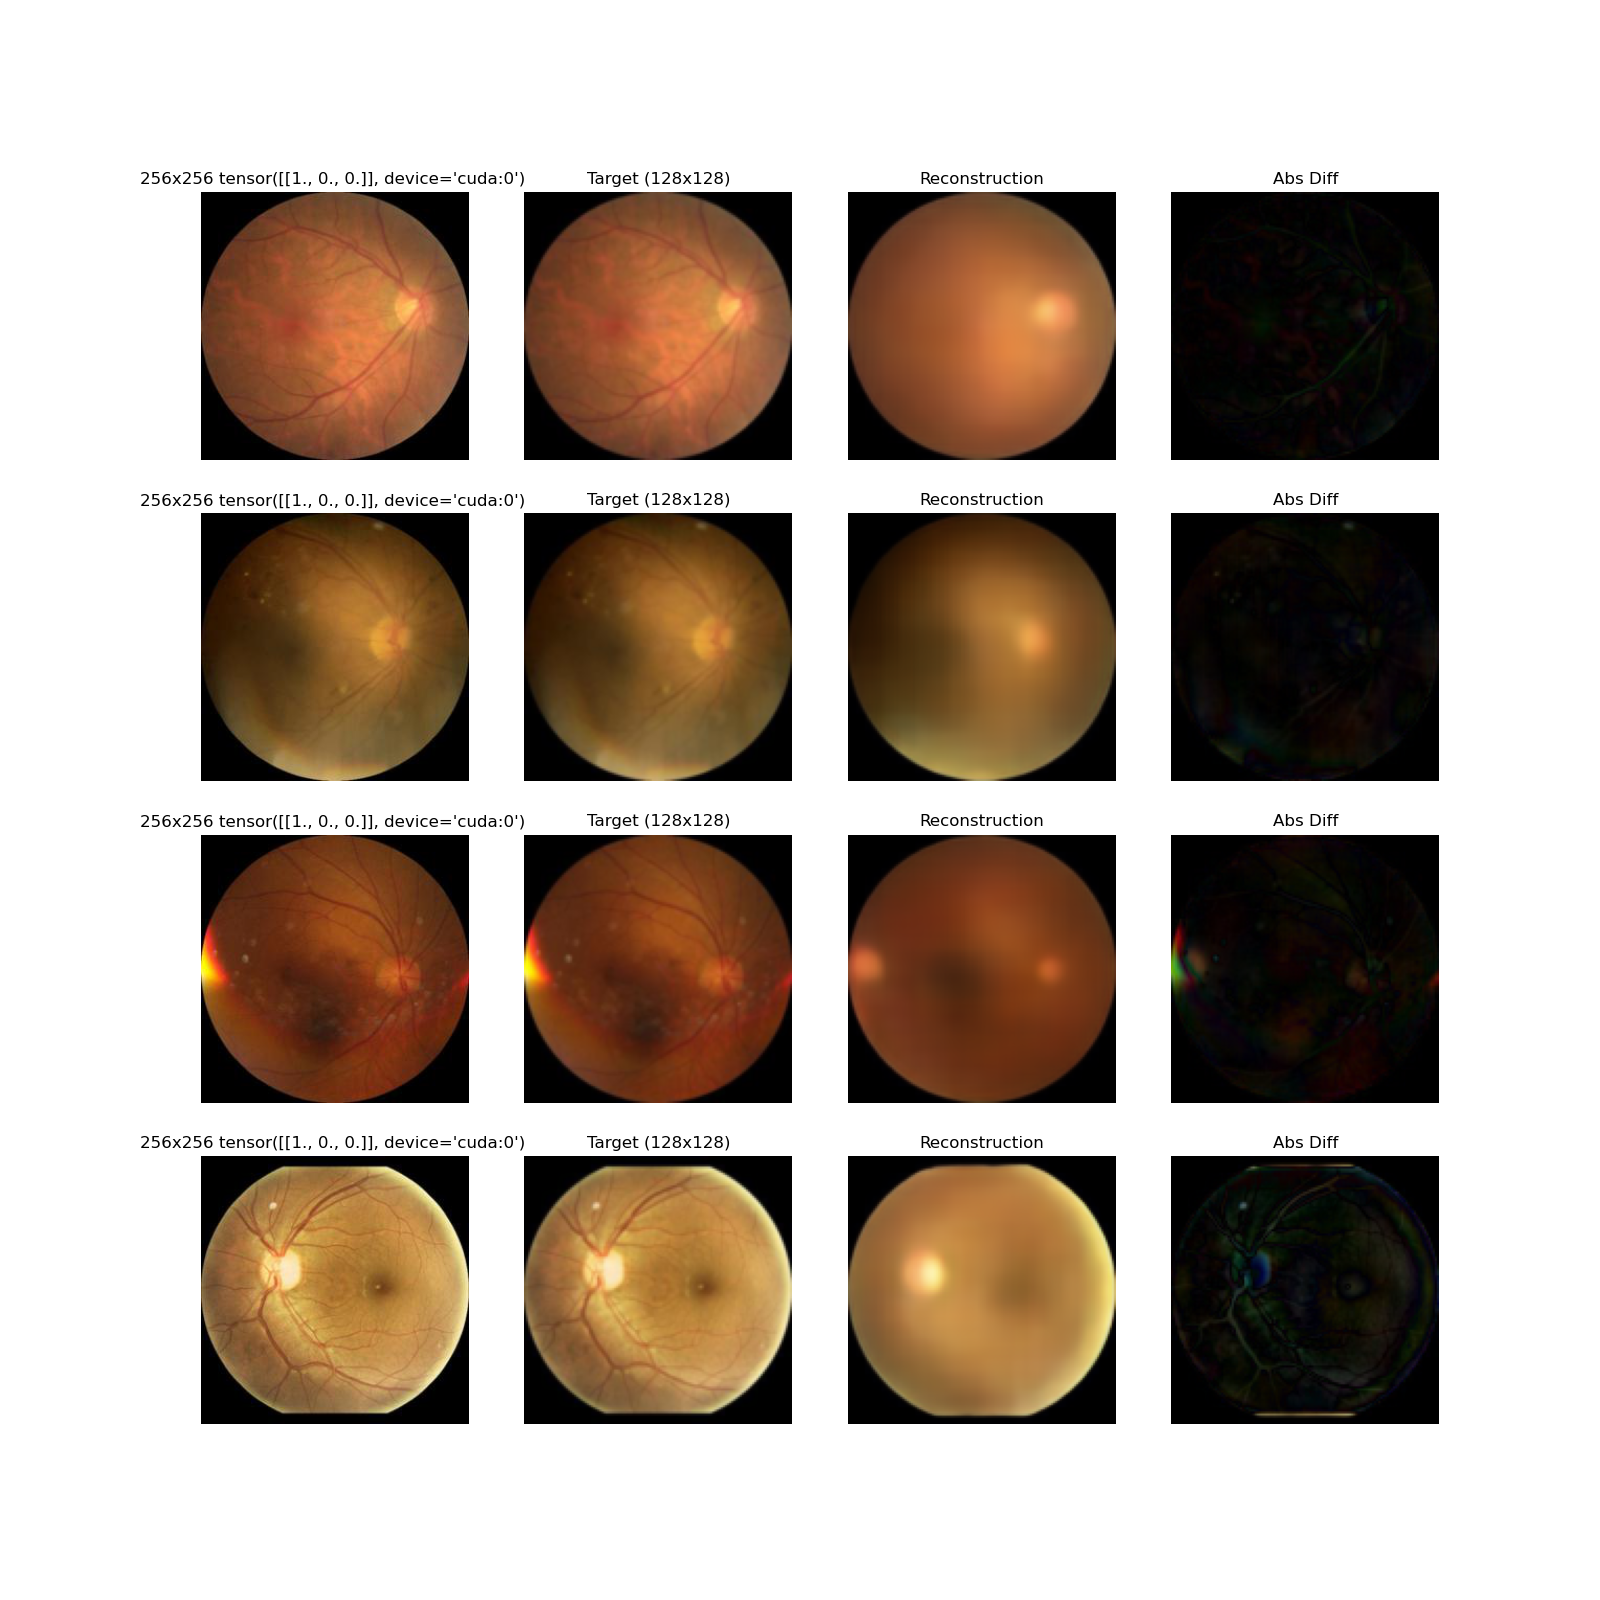
\includegraphics[width=1\linewidth]{recon.png}
    \caption{cVAE reconstructions}
    \label{fig:recon}
\end{figure}
\begin{figure}[!ht]
    \centering
    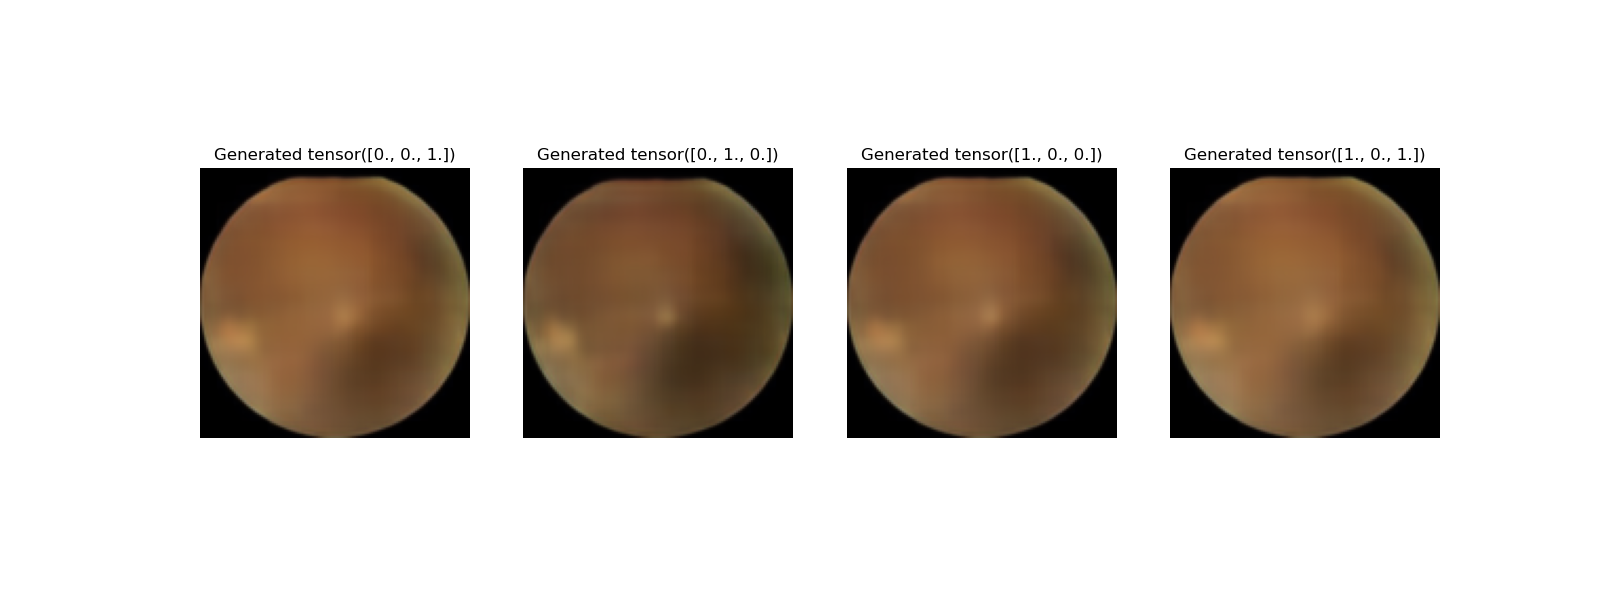
\includegraphics[width=1\linewidth]{cvae_generated.png}
    \caption{cVAE class-conditional generation}
    \label{fig:cvae_generated}
\end{figure}
\begin{figure}[!ht]
    \centering
    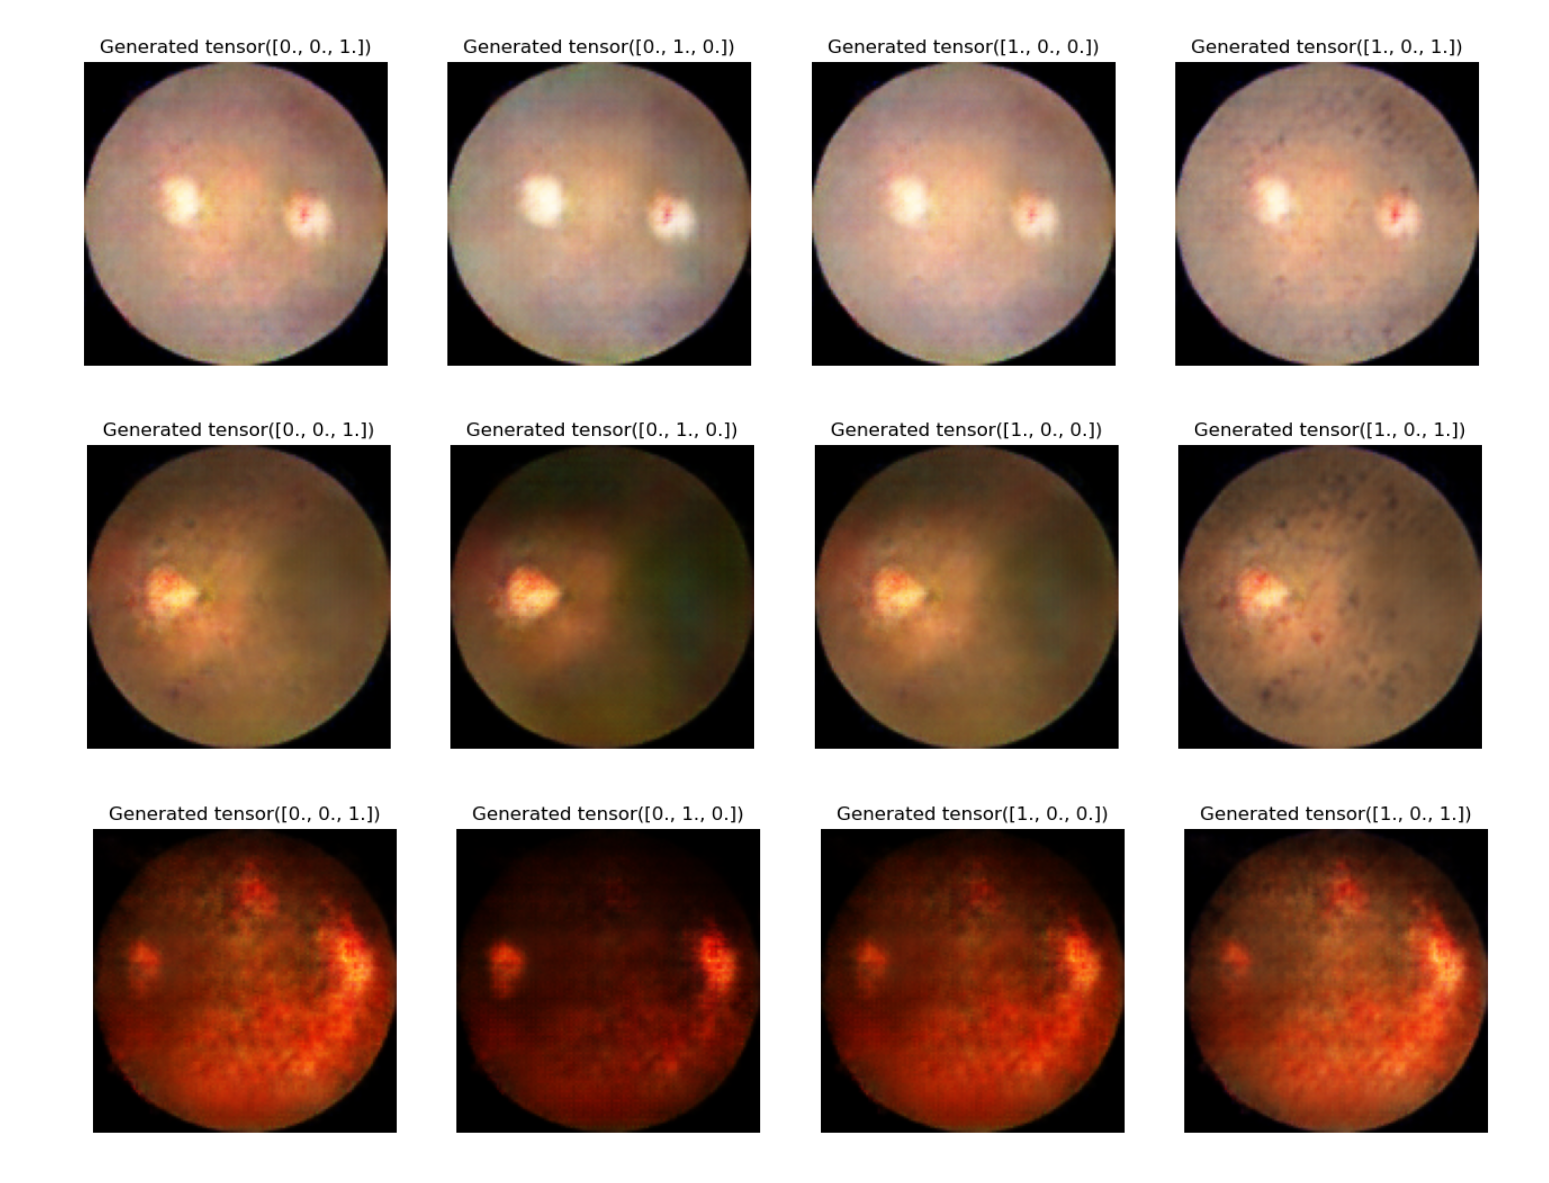
\includegraphics[width=1\linewidth]{gan_gen.png}
    \caption{Conditional DCGAN generated images}
    \label{fig:gan_gen}
\end{figure}

\counterwithin{figure}{section}
\begin{figure}[H]
    \centering
    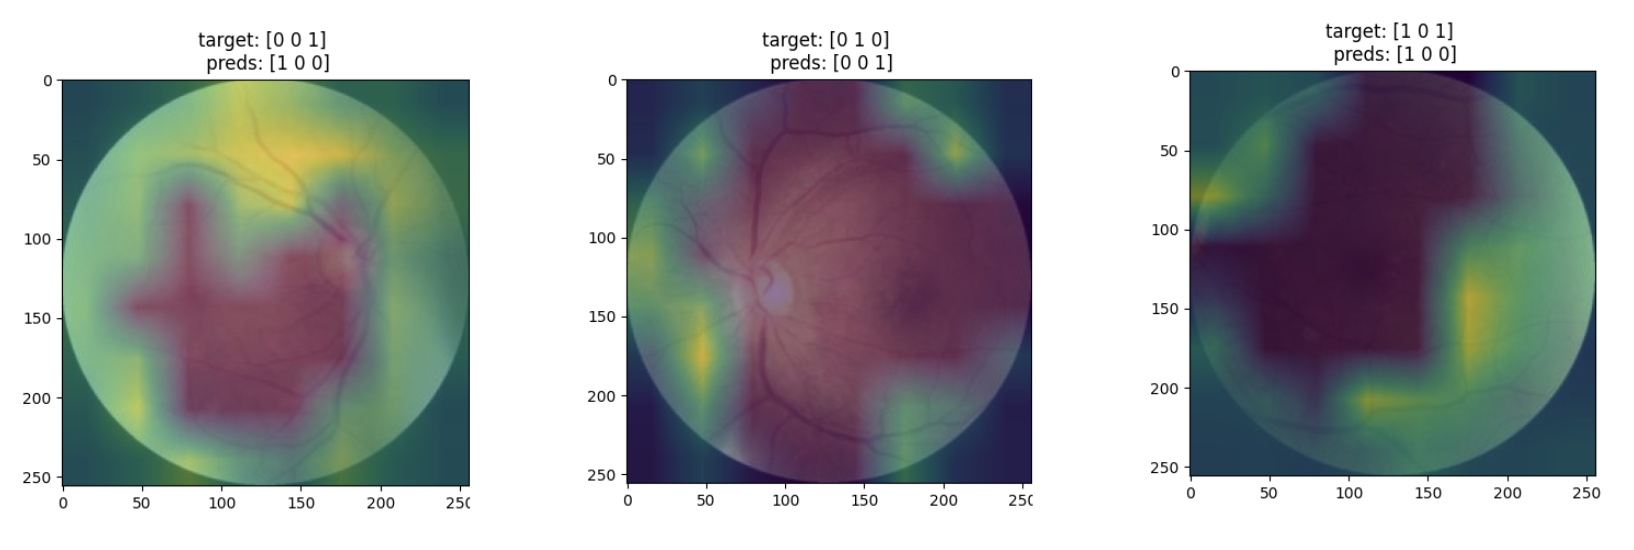
\includegraphics[width=1\linewidth]{grad-cam-augment.png}
    \caption{Grad-CAM overlay observations to add noise augmentation}
    \label{fig:grad-cam-augment}
\end{figure}

\section{Tuning settings}
\label{app:settings}
\begin{table}[H]
\centering
\begin{tabular}{lcccc}
\toprule
\textbf{Stage} & \textbf{LR}  & \textbf{WD} & \textbf{Schedule} & \textbf{Epochs} \\
\midrule
Head
& $10^{-3}$ & $10^{-4}$
& $Step=8$, $\gamma=0.8$
& 20 \\
Full
& $5{\times}10^{-4}$ & $10^{-4}$
& Exp: $\gamma=0.2$
& 5 \\
\bottomrule
\end{tabular}
\caption{Bare ResNet18 (AdamW).}
\label{tab:resnet_training_schedule}
\end{table}
\begin{table}[H]
\centering
\begin{tabular}{lcccc}
\toprule
\textbf{Stage} & \textbf{LR}  & \textbf{WD} & \textbf{Schedule} & \textbf{Epochs} \\
\midrule
Head
& $10^{-3}$ & $10^{-4}$
& $Step=10$, $\gamma=0.8$
& 20 \\
Full
& $5{\times}10^{-4}$ & $0$
& Exp: $\gamma=0.2$
& 5 \\
\bottomrule
\end{tabular}
\caption{Bare EfficientNetB0 (AdamW)}
\label{tab:efficientnet_training_schedule}
\end{table}

\begin{table}[H]
\centering
\begin{tabular}{lcccc}
\toprule
\textbf{Stage} & \textbf{LR} & \textbf{WD} & \textbf{Schedule} & \textbf{Epochs}\\ 
\midrule
Block
& $10^{-3}$
& $10^{-4}$
& Step: $8$, $\gamma=0.7$
& 20 \\
Full
& $5{\times}10^{-4}$
& $10^{-4}$
& Exp: $\gamma=0.5$
& 5 \\
\bottomrule
\end{tabular}
\caption{EfficientNetB0 + SE (AdamW).}
\label{tab:efficientnet_se_training_schedule}
\end{table}

\begin{table}[H]
\centering
\begin{tabular}{lcccc}
\toprule
\textbf{Stage} & \textbf{LR} & \textbf{WD} & \textbf{Schedule} & \textbf{Epochs}\\ 
\midrule
Block
& $5{\times}10^{-4}$
& $10^{-5}$
& Cosine: $T_{\max}=5$
& 20 \\
Full
& $10^{-3}$
& $10^{-4}$
& Exp: $\gamma=0.5$
& 10 \\
\bottomrule
\end{tabular}
\caption{EfficientNetB0 + Transformer block (AdamW)}
\label{tab:efficientnet_mha_training_schedule}
\end{table}

\begin{table}[H]
\centering
\begin{tabular}{lcccc}
\toprule
\textbf{Stage} & \textbf{LR} & \textbf{WD} & \textbf{Schedule} & \textbf{Epochs}\\
\midrule
Head
& $10^{-4}$
& $10^{-4}$
& $Step=8$, $\gamma=0.8$
& 20 \\
Full
& $3{\times}10^{-4}$
& $10^{-4}$
& Exp: $\gamma=0.7$
& 10 \\
\bottomrule
\end{tabular}
\caption{ResNet18 + Focal Loss (AdamW)}
\label{tab:resnet_focal_training_schedule}
\end{table}

\begin{table}[H]
\centering
\begin{tabular}{lcccc}
\toprule
\textbf{Stage} & \textbf{LR} & \textbf{WD} & \textbf{Schedule} & \textbf{Epochs}\\
\midrule
Head
& $10^{-3}$
& $10^{-4}$
& $Step=8$, $\gamma=0.8$
& 20 \\
Full
& $5{\times}10^{-4}$
& $10^{-4}$
& Exp: $\gamma{=}0.5$
& 5 \\
\bottomrule
\end{tabular}
\caption{ResNet18 + WBCE (AdamW)}
\label{tab:resnet_wbce_training_schedule}
\end{table}

\begin{table}[H]
\centering
\begin{tabular}{lcccc}
\toprule
\textbf{Stage} & \textbf{LR} & \textbf{WD} & \textbf{Schedule} & \textbf{Epochs} \\
\midrule

Grad-CAM
& $10^{-3}$
& $10^{-4}$
& Exp: $\gamma=0.5$
& 20 \\
\bottomrule
\end{tabular}
\caption{EfficientNet fine-tuning with Grad-CAM–based explanation loss (AdamW).}
\label{tab:efficientnet_gradcam_training}
\end{table}


\begin{table}[H]
\centering
\begin{tabular}{lccccc}
\toprule
\textbf{Stage} & \textbf{LR} & \textbf{WD} & \textbf{Schedule} & \textbf{Epochs} \\
\midrule
Head
& $3{\times}10^{-4}$
& $10^{-3}$
& $Step=5$, $\gamma=0.8$
& 10 \\
Full 
& $3{\times}10^{-5}$
& $10^{-4}$
& $Step=5$, $\gamma=0.5$
& 30 \\
\bottomrule
\end{tabular}
\caption{SwinV2-Tiny (AdamW)}
\label{tab:swin_training_schedule}
\end{table}

\begin{table}[H]
\centering
\begin{tabular}{lc}
\toprule
\textbf{Setting} & \textbf{Value} \\
\midrule
Optimizer & Adam \\
Learning rate & $10^{-4}$ \\
KL warm-up & 100 epochs \\
Max KL coefficient $\beta$ & 1.0 \\
Epochs & 450 \\
\bottomrule
\end{tabular}
\caption{Training configuration for the cVAE.}
\label{tab:cvae_training}
\end{table}

\begin{table}[H]
\centering
\begin{tabular}{lc}
\toprule
\textbf{Setting} & \textbf{Value} \\
\midrule
Optimizer ($G$, $D$) & Adam \\
Learning rate ($G$) & $5{\times}10^{-5}$ \\
Learning rate ($D$) & $10^{-4}$ \\
Adam $(\beta_1, \beta_2)$ & $(0.5,\ 0.999)$ \\
Epochs & $>$1000\\
\bottomrule
\end{tabular}
\caption{Training configuration for the cDCGAN.}
\label{tab:dcgan_training}
\end{table}


\end{document}
